\documentclass[12pt,a4paper]{article}
\usepackage[utf8]{inputenc}
\usepackage{amsmath}
\usepackage{amsfonts}
\usepackage{amssymb}
\usepackage{color}
\author{Zhuoran Liu}
\title{Multi-Layer Perceptron}
\usepackage{graphicx}

\begin{document}
\maketitle

\color{black}
\newpage
\section{Introduction}
In this report, we will consider the neural network multi-layer perceptron. Multi-layer perceptron is a neural network with multiple hidden layers and in each hidden layer there are multiple neurons. Between different neurons in adjacent layers, there exist weights to connect different neurons. In every hidden layer, there exist biases to tune some outcomes of neurons. The aim of training the network is to find the proper weights and biases which can be used to predict the new data.
\subsection{Underlying Theory}
Firstly, we will talk about the working mechanism of the MLP. Given the neural network structure(weights matrix $W$ and biases vector $b$) and input data vector $a$, we can calculate the feed forward process by formula
\[\textbf{z} = g(\textbf{w}a + \textbf{b})\]
Here $g$ is the activation function and output $z$ is a vector. Use $z$ as the input of the next layer, we can do similar calculation again until we get the output. Given the last output $z$, we will calculate the $argmax(z)$. The category of the $argmax(z)$ is the predication of the input $a$. Known the right category, we will tune the weights and biases to predict better and better. This is the learning process of MLP. 
Given the input 
\subsection{Learning Algorithm}
Backpropagation algorithm is the learning algorithm we will use. It consists of 4 steps.
\[\delta^L = \nabla_{a} C \circ \sigma'(z^{L})\]
\[\delta^L = ((w^{l+1})^{T} \delta^{l+1} \circ \sigma'(z^{l})\]
\[\frac{\partial C}{\partial b_{j}^{l}} = \sigma_{j}^{l}\]
\[\frac{\partial C}{\partial w_{jk}^{l}} = a_{k}^{l-1} \sigma_{j}^{l}\]
This four step will backpropagate error and output the gradient change of cost function. The whole process is input, feedforward, backpropagate, update weights and biases, input again... Finally after many epoches we will get the final neural network with particular weights and biases, then we finish training.
\newpage
\section{Problem statement}
1. The influence of different layers and different number of neurons.\\
2. The different initializations of the weights and biases before learning.\\
3. Different chooses of activation functions.\\
4. different learning method Stochastic Gradient Descent vs. Momentum.\\
\section{Results}
\subsection{The structure of Multi-Layer Perceptron}
\subsubsection{Different neurons}
The first problem to investigate is the influence on classification accuracies from the number of neurons in hidden layers. We did the experiment with five different settings. All the settings have one hidden layer with different neurons. All five experiments used same input layer ($784$) and output layer, and used same epoches (1$50$), same learning rate ($0.05$) and same mini-batch number ($10$). The plot below shows the results of five different setting.Blue line is $2$ neurons, red line is $5$ neurons, black line is $10$ neurons, green line is $20$ neurons and magenta line is $100$ neurons.\\
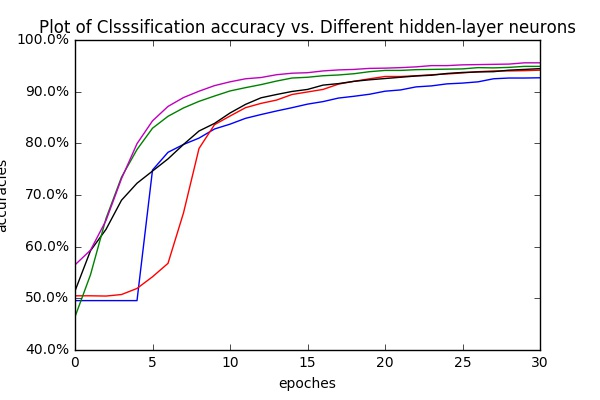
\includegraphics[width=90mm,scale=1]{p101.jpg}\\
The horizontal axis showed the epoches changed from $0$ to $150$, and the vertical axis showed the test accuracies in percentage. The formula is
\[\text{accuracy} = \frac{\text{right classified number in test images}}{ \text{total number in test images}}\]\\
From the plot we can easily see that, if there is one hidden layer, more hidden neurons will yield better results. But in small amount of epches, less neurons may have better results. For example, blue line is better than red and black in epoch $6$.\\
More neurons will take more training time, and the relationship between neurons and time are almost linear. The plot below is the running time of the five experiments we mentioned above.\\
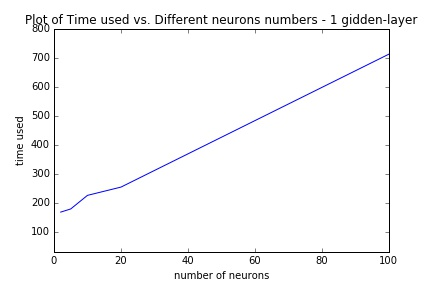
\includegraphics[width=90mm,scale=1]{p102.jpg}\\
From this figure, we can easily see that the relationship between neurons and time is almost linear.
\subsubsection{Different layers}
The second problem to investigate is the influence on classification accuracies from the number of hidden layers. We did the experiment with five different settings. The settings of hidden layer number ranges from $1$ to $5$, and in each hidden layer we used $5$ neurons. All five experiments used same input layer ($784$) and output layer, and used same epoches ($100$), same learning rate ($0.05$) and same mini-batch number ($10$). The plot below shows the results of five different settings.\\
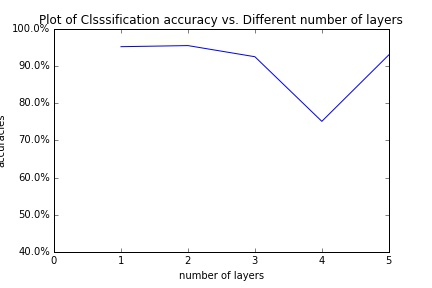
\includegraphics[width=90mm,scale=1]{p103.jpg}\\
From the figure, we can see that $4$ hidden layers had a bad performance. The other experiments almost performed the same. This problem may be caused by the training data. Since we just need to classify number $3$ and number $7$, so no more complicated model should be trained. So more layers didn't perform better.\\
More layers will take more training time, and the relationship between layers' number and time are almost linear. The plot below is the running time of the five experiments we mentioned above.\\
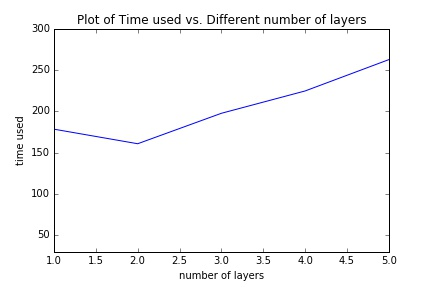
\includegraphics[width=90mm,scale=1]{p104.jpg}\\
From this figure, we can easily see that the relationship between number of layers and time is almost linear.

\subsection{The initialization of the weights and biases}
By default we choose the initialization of weights and biases using Gausssian random variables with mean $0$ and deviation $1$. Here we used another way to improve it such that we can have a better initialization and better results.
\subsubsection{different initialization of weights and biases}
Here we mainly considered the initialization with a normalized Gaussian. The formula is\\
\[\text{initialization of weights}= \frac{\text{random} (y, x)}{\sqrt{x}}\]\\
This setting can make the distribution more sharply peaked whcih makes it less likely that neuron will saturate. We did experiment for both initializations and have the results below.Both experiments used same input layer ($784$) and output layer, and used same epoches ($150$), same learning rate ($0.05$) and same mini-batch number ($10$).Both with $1$ hidden layer and $100$ neurons. The plot below shows the results of two different settings.\\
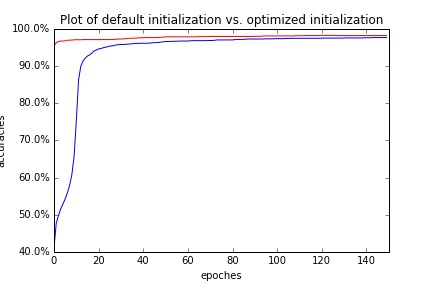
\includegraphics[width=90mm,scale=1]{p201.jpg}\\
From the figure, we can easily see that. Optimized initialization with a normalizing component will make the initial accuracy munch higher than the default gaussian distribution. Also it showed a better result than the default setting.
\subsubsection{different activation functions}
By default we used sigmoid function as the activation function. Here we compared the sigmoid function with tanh function.\\
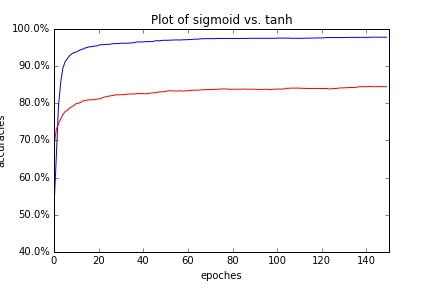
\includegraphics[width=90mm,scale=1]{p301.jpg}\\
From this figure we can see that sigmoid did better, since the initialization is better.\\
With better initialization of tanh!!


\subsection{Different learning methods}
\subsubsection{Stochastic gradient descent vs. Momentum}
Momentum is a method to escape from local minimum, and it did speed up the learning process by changing gradient direction more straight forward to the target. We used two formulas to implement the momentum learning.
\[v' = \mu v - \eta \nabla C\]
\[w' = w + v'\]
After implementation we got the results compared with stochastic gradient method as below.\\
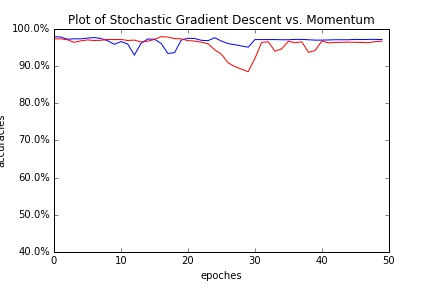
\includegraphics[width=90mm,scale=1]{p401.jpg}\\
From this figure, we can easily see that momentum(blue) convergence faster??



\section{Discussion}


\section{Conclusion}
Multi-layer perceptron is perceptron which can be trained by various patterns. It is not easy to be trained well. This training process depended on many aspects. For example number of neurons, number of layers, initialization of weights and biases, exact learning method, learning rate, size of mini-batches and so on. 
From what we have explored, more hidden layers and more neurons involved will have better results, but it will also take more time. The time has a similar linear relationship with the number of neurons and the number of hidden layers. A good initialization can obviously improve the initial accuracy of the learning process, and it also help tune the weights and biases better. Different activation functions have different influences on the accuracies of test, and they have also different running time. The choose of learning rate, epoches and mini batch sizes are also import parts. But they can be investigated by some experiments and choose the comparable better one.

\newpage
\section{Appendix}
\end{document}